\section{Introduction}
\label{sec:introduction}

As conversational Large Language Models (LLMs) are deployed in sensitive domains such as customer support, clinical workflows, and autonomous agent loops, verifying that conversational outputs adhere to safety standards is a critical operational requirement. While human moderation remains the authoritative gold standard, manual auditing cannot scale to continuous production throughput. Consequently, automated evaluation pipelines—popularized under the \textit{LLM-as-a-judge} paradigm~\cite{chiang2023vicuna,zheng2023judging,wang2023pandalm}—are widely adopted to evaluate dialogues and detect safety violations~\cite{zhang2024safetybench,mazeika2024harmbench}.

Standard LLM-as-a-judge pipelines rely almost exclusively on commercial cloud-hosted frontier models or massive open-weight clusters ($70\text{B}+$ parameters)~\cite{touvron2023llama,tan2025judgebench,bavaresco2025llms}. While effective, this centralized paradigm introduces significant operational friction:
\begin{enumerate}
    \item \textbf{Data Confidentiality and Compliance:} Transmitting conversational transcripts to third-party cloud APIs creates ongoing compliance overhead under data protection frameworks such as GDPR and HIPAA~\cite{debenedetti2024evading}. Local on-premises inference preserves internal data perimeters.
    \item \textbf{Economic and Throughput Overhead:} High-volume offline auditing incurs recurring token costs and rate-limiting bottlenecks.
    \item \textbf{Logit Obfuscation:} Commercial APIs frequently withhold token logit distributions, preventing downstream systems from extracting continuous probability estimates or assessing predictive confidence.
\end{enumerate}

These constraints motivate investigating \textit{small open-weight language models} (SLMs) with fewer than 2 billion parameters~\cite{yang2024qwen25,allal2025smollm2} as localized safety evaluators. Sub-2B models can execute deterministically on commodity x86 CPUs within bounded memory footprints ($<1.2\text{ GB}$ peak resident set size), enabling self-contained edge evaluation without dedicated GPUs.

\begin{figure}[t]
    \centering
    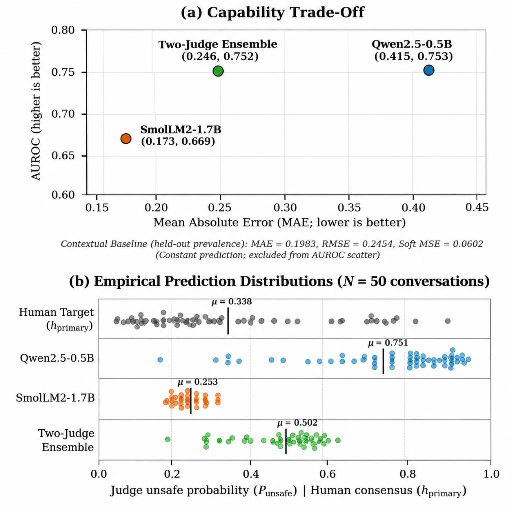
\includegraphics[width=\columnwidth]{figures/fig1_tradeoff.pdf}
    \caption{Evaluator polarization and ensembling trade-offs on an exploratory sample of $N=50$ multi-turn adversarial conversations from Google DICES-350. (a) Capability trade-off plane: Mean Absolute Error (MAE, lower is better) versus majority-consensus discrimination ($\text{AUROC}$, higher is better). Qwen2.5-0.5B achieves strong ranking sensitivity ($\text{AUROC} = 0.7529, \rho = 0.5680$) but severe overprediction ($\text{MAE} = 0.4152$). SmolLM2-1.7B achieves the lowest judge MAE ($0.1734$) but compressed ranking acuity ($\text{AUROC} = 0.6690, \rho = 0.3929$). The Two-Judge Ensemble provides an empirical compromise, cutting Qwen's MAE by $40.6\%$ while capturing the highest rank correlation ($\rho = \mathbf{0.5903}$) and preserving AUROC ($0.7517$). A naive held-out prevalence baseline achieves the lowest squared error ($\text{Soft MSE} = 0.0602$). (b) Prediction distributions ($N=50$) illustrating Qwen's risk-averse bias ($\mu = 0.751$) and SmolLM2's variance compression ($\sigma = 0.039$) around human consensus prevalence ($0.338$).}
    \label{fig:tradeoff}
\end{figure}

However, small models exhibit severe susceptibility to inductive bias, probability miscalibration, and sensitivity to prompt formulation~\cite{tan2025judgebench,schwinn2026coin}. Recent work demonstrates that automated judges can collapse toward chance accuracy when evaluating adversarial inputs~\cite{schwinn2026coin}. Furthermore, existing benchmarks collapse multi-rater evaluations into binary labels, discarding the continuous distribution of human judgment~\cite{aroyo2023dices,davani2022dealing,rottger2022two}. In classical machine learning, ensembling diverse models mitigates inductive bias and improves calibration~\cite{lakshminarayanan2017simple,ovadia2019can}. While multi-agent jury architectures have been explored for frontier models~\cite{verga2024replacing,qian2026who}, whether heterogeneous sub-2B models running on commodity CPUs can reliably approximate continuous human safety consensus remains unexplored.

To address this gap, we present \textbf{TrustEval}, an empirical study evaluating the representational accuracy, ranking discrimination, calibration behaviour, and error-uncertainty dynamics of sub-2B open-weight safety judges. We examine an equal-weight ensemble of two structurally distinct architectures—\texttt{Qwen2.5-0.5B-Instruct} (0.49B) and \texttt{SmolLM2-1.7B-Instruct} (1.71B)—evaluated on 50 multi-turn adversarial dialogues from Google DICES-350~\cite{aroyo2023dices}. Each conversation features ratings from 104 retained crowd raters ($5,200$ total evaluations), enabling direct evaluation against continuous human consensus proportions ($h_{\text{primary}} \in [0, 1]$). Furthermore, we examine whether inter-judge disagreement ($\Delta = |P_{\text{qwen}} - P_{\text{smol}}|$) serves as an informative candidate correlate for ensemble evaluation error.

As shown in Figure~\ref{fig:tradeoff}, our results reveal a pronounced trade-off: Qwen provides strong hazard discrimination alongside aggressive overprediction, whereas SmolLM2 achieves low point error via variance compression around benchmark prevalence. An unweighted ensemble negotiates this frontier, moderating prediction error relative to Qwen while improving rank correlation over both individual judges.

\subsection{Research Questions}
\label{sec:rqs}

This paper investigates three primary research questions:
\begin{itemize}
    \item \textbf{RQ1 (Point Error and Calibration):} Can sub-2B open-weight LLMs running on commodity CPUs approximate continuous human safety consensus, and how does an equal-weight ensemble compare against individual constituent judges and naive prevalence baselines in MAE, RMSE, Soft MSE, and decile calibration ($\text{ECE}_{10}$)?
    \item \textbf{RQ2 (Discriminative Hazard Ranking):} How do compact judges and their ensemble perform in ranking conversational hazard relative to human consensus (Pearson $r$, Spearman $\rho$, AUROC), and does ensembling preserve discriminative sensitivity while tempering single-model bias?
    \item \textbf{RQ3 (Disagreement as an Error Correlate):} Does inter-judge disagreement ($\Delta$) provide an informative candidate signal for ensemble error, accounting for variance beyond response length and predicted probability?
\end{itemize}

\subsection{Summary of Contributions}
\label{sec:contributions}

The primary contributions of this paper are:
\begin{enumerate}
    \item \textbf{Continuous Multi-Rater Evaluation Benchmark:} We provide an empirical evaluation of sub-2B open-weight LLMs tasked with predicting continuous human safety consensus ($h_{\text{primary}} \in [0, 1]$) derived from 104 crowd annotators per item across 50 adversarial dialogues from Google DICES-350 ($5,200$ total ratings).
    \item \textbf{Characterization of Single-Judge Trade-Offs:} We demonstrate pronounced evaluator polarization: Qwen2.5-0.5B achieves high ranking sensitivity ($\text{AUROC} = 0.7529, \rho = 0.5680$) but exhibits substantial overprediction bias ($\bar{P} = 0.7509$ vs. human mean $0.3381$) and miscalibration ($\text{ECE}_{10} = 0.4128$). Conversely, SmolLM2-1.7B achieves the lowest sample MAE ($0.1734$) via variance compression ($\sigma = 0.0388$) near sample prevalence ($0.3381$), with modest discrimination ($\text{AUROC} = 0.6690, \rho = 0.3929$).
    \item \textbf{Empirical Trade-Off Expansion via Ensembling:} We show that an equal-weight ensemble synthesizes these behaviors, cutting Qwen's MAE by $40.6\%$ (to $0.2464$, $p = 1.04 \times 10^{-7}$) and Soft MSE by $67.6\%$ ($p = 2.85 \times 10^{-9}$) while maintaining majority discrimination ($\text{AUROC} = 0.7517$) and achieving the highest linear ($r = \mathbf{0.4992}$) and rank correlation ($\rho = \mathbf{0.5903}$). We document that ensembling represents an operational trade-off rather than universal dominance: SmolLM2 achieves lower sample MAE, and the ensemble remains systematically overpredicting ($\text{ECE}_{10} = 0.1639$).
    \item \textbf{Prevalence Baseline Reality Check:} We document that a naive 5-fold held-out prevalence baseline achieves the lowest overall squared error ($\text{Soft MSE} = 0.0602$), outperforming all evaluated models, highlighting the challenge small models face under quadratic loss.
    \item \textbf{Empirical Audit of Inter-Judge Disagreement:} We find that inter-judge disagreement ($\Delta$) shows a nominally significant positive association with ensemble error ($r = 0.3125, p = 0.0271$; nested OLS $F(1, 46) = 5.676, p = 0.0214$). We demonstrate that while disagreement is an informative candidate signal, low disagreement does not guarantee correctness due to potential shared inductive biases.
    \item \textbf{Edge-Inference Profiling:} We demonstrate that deterministic logit scoring executes locally on commodity x86 CPUs within bounded memory footprints ($<1.2\text{ GB}$ peak RSS), establishing the feasibility of decentralized safety auditing.
\end{enumerate}
